\documentclass{../local}

\begin{document}
In voorgaande hoofdstuk is de herkomst van de  opdracht beschreven. In dit hoofdstuk wordt het project en de opdracht gedefinieerd en gedetailleerd beschreven.

\section{Projectomvang}
Het project zal worden uitgevoerd door 1 persoon, de afstudeerder. Het project is van een bepaalde tijd, namelijk van 3 maart 2014 tot en met 8 juli 2014. Dit houdt in dat er in totaal 720 uur beschikbaar is.

De afstudeerder zal worden bijgestaan door Martin Klomp als bedrijfsbegeleider van Alten PTS. Vanuit de Hogeschool Utrecht zal Leo van Moergestel de afstudeerder bijstaan als docentbegeleider. In bijlage A is er bedrijf- en persoonsgegevens van de betrokkenen te vinden.

\section{Opdracht}
Vanuit het oogpunt van het project 'Veiligheid op de werkvloer', de interesses van de student en als meerwaarde voor Alten PTS, is de volgende opdracht geformuleerd: \\
\textbf{Het maken van een gedistribueerde Wireless Sensor Netwerk (WSN) die helpt bij het navigeren van personen bij een noodsituatie, zoals een branduitbraak of ontsnapping van een gevaarlijk gas.}

\section{Doelstellingen}

Het doel van dit project is om een functioneel demonstratie model (demonstrator) te hebben voor Alten PTS dat getoond kan worden aan potentiële klanten die geïnteresseerd zijn in oplossingen voor 'veiligheid op de werkvloer'. In het geval van dit project is de demonstrator een WSN die een navigatie toont bij een noodsituatie. De navigatie en noodsituatie detectie mag een simpele werking hebben (gebruik van LED's of drukknoppen). Deze demonstrator moet werkend zijn op fysieke hardware. 

Hoewel dit project een onderdeel is van het project 'veiligheid op de werkvloer', is het goed om een doelstelling te definiëren voor het product zelf. De doelstelling van dit product is om aan te tonen dat het gebruik van een WSN als systeem voor gevaardetectie (brand) en evacuatienavigatie voor personen een haalbaar concept is.

Als uitbreiding op deze doelstelling kan het WSN na een evacuatie aanwezige reddingswerkers dienen door sensor informatie door te sturen naar mobiele ontvangers. Hierdoor is het mogelijk dat de reddingswerker een verwachting heeft over de komende situatie, of een ideale route kan geven naar een bepaalde locatie. Ook kan de reddingswerker tegelijkertijd gevolgd worden vanaf een basisstation \cite{ShaWSN}.

\section{Scope}
In voorgaande sectie is de opdracht gedefinieerd. In deze sectie wordt deze opdracht afgebakend. Er worden aannames gemaakt en aangegeven aan welk onderdeel wordt gewerkt en aan welk onderdeel niet wordt gewerkt.

Dit project zal zich focussen op het maken van een demonstrator. Dit impliceert dat er software gemaakt wordt wat draait op fysieke hardware om te kunnen worden getoond. In dit project wordt de focus op het maken van deze software gelegd. Problemen of aandachtspunten voor hardware wordt zo min mogelijk naar gekeken om het project haalbaar te maken.

\begin{itemize}
\item Nodes zijn zo ontworpen dat deze op elke locatie kan worden geplaatst. Ook op locaties waar niet een vaste stroomvoorziening is. De nodes moeten dan op batterij draaien. Bij het ervan moet dan ook altijd het stroomverbruik in acht genomen worden. In dit project wordt hier geen rekening mee gehouden. Er wordt aangenomen dat er altijd stroomvoorziening is. Ook hoeven er geen optimalisaties worden gedaan om het stroomverbruik zo min mogelijk te houden.

\item Bij WSN's wordt er uiteraard met draadloze verbindingen gewerkt. Draadloze netwerken hebben 
redelijk complexe technieken onder de motorkap om het zo optimaal mogelijk werkend te hebben. Tegenwoordig zijn er genoeg platformen beschikbaar die een startende ontwikkelaar met gebruik van WSN's een snelle start geven. Voorbeelden van deze platformen zijn: Zigbee\footnote{\url{www.zigbee.org/}}, Tiny OS\footnote{\url{www.tinyos.net/}}, Contiki OS\footnote{\url{www.contiki-os.org/}} en RIOT OS \footnote{\url{www.riot-os.org/}}. Deze platformen geven ondersteuning voor het opzetten van draadloze netwerken en er zijn veel voorbeelden beschikbaar. Ook geven deze platformen functionaliteit om makkelijker met embedded apparaten te werken. Dit project zal een van deze platformen gebruiken. 

\item Om de demonstratie zijn kracht goed toonbaar te maken, moeten er meerdere nodes binnen het WSN gebruikt worden. Initieel wordt gedacht om 5 nodes te gebruiken voor het demonstratie model.

\item De veiligheid van systemen tegen kwaadwillenden is iets wat tegenwoordig hoog in het vaandel staat. Dit project zal geen rekening houden met de beveiliging van het systeem. Aangezien het een demonstratiemodel is, is dat ook niet nodig. Bij live gebruik van het systeem is dat noodzakelijk.

\item Een veiligheidssysteem die bedoeld is om mensenlevens te redden moet zeer strenge regels opvolgen om te mogen dienen in gebouwen. Het systeem moet uitmuntend robuust zijn en een zeer goed reactievermogen hebben. In dit project zal hier zoveel mogelijk naar gekeken worden, maar niet garantie geven op het voldoen van de hoge eisen. In sectie kwaliteitscriteria wordt hierover meer beschreven.

\item In dit project gaat het vooral om het ontwikkelen van de software. Hiermee zeggende zal de focus bij het maken van de software ook liggen op de architectuur/structuur van de software.
\end{itemize}

\section{Requirements}
In voorgaande secties is de opdracht gedefinieerd en afgebakend. In deze sectie zal er requirements aan het systeem gesteld worden. Deze requirements zijn opgesteld volgens de MoSCoW methode.
\\\\

\begin{wrapfigure}[13]{r}{0.4\textwidth}
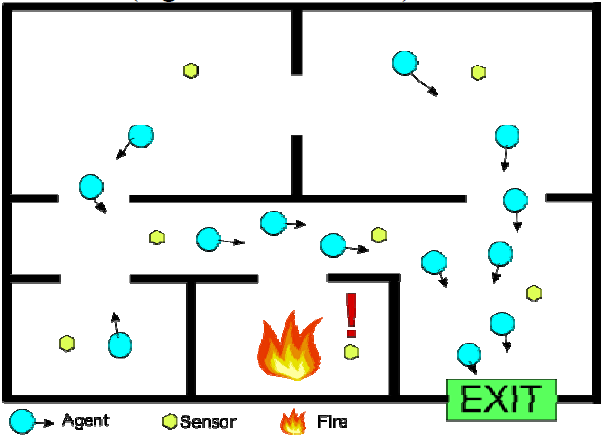
\includegraphics[width=7cm]{../images/BrandNavigatieVoorbeeld}
\caption{\emph{Voorbeeld routebepaling bij brand\cite{ZengFire}}}
\end{wrapfigure}

\noindent\textbf{Must Have}
\begin{itemize}
\item Het WSN moet dienen als een brand detectie systeem.
\begin{itemize}
\item De nodes hoeven niet een hoogwaardig branddetectiesysteem te hebben, voor de demonstratie opstelling is een schakelaar of knop genoeg.
\end{itemize}
\item Het WSN moet bij een brandmelding een route op basis van soort gevaar naar de uitgang tonen die de gevaarlijke zones vermijdt. Een voorbeeld kan worden gezien in Figuur 2.1. Hierin geven agents, die gezien kunnen worden als navigatiepanelen, aan waar heen moet worden gelopen. Er zijn sensoren aanwezig en een sensor heeft een brand gedetecteerd.
\begin{itemize}
\item Voor demonstratie doeleinden hoeft de aanduiding van de route d.m.v. de nodes niet direct intuïtief te zijn. Aangeven door middel van LED's kan genoeg zijn of een via een PC.
\end{itemize}
\end{itemize}

\begin{itemize}
\item Om het decentrale gedeelte van het WSN wezenlijk te maken, moet elke node zijn eigen route berekenen.

\item Het WSN moet een robuust netwerk zijn. Dat wil zeggen dat wanneer er een node uitvalt binnen het WSN, het volledige systeem niet mag uitvallen.
\end{itemize}

\noindent\textbf{Should Have}
\begin{itemize}
\item Meerdere soorten gevaren detecteren dan alleen brandgevaar. Hiervoor kan een abstractielaag voor worden ontworpen. De routebepaling moet per soort gevaar te definiëren zijn.
\item Een systeem die de status van de nodes kan monitoren. Te monitoren waardes zullen zijn:
\begin{itemize}
\item Status van de node (operationeel, defect, etc.).
\item Aangegeven bepaalde navigatie wanneer de noodtoestand bezig is.
\item Sensor data.
\end{itemize}
\end{itemize}

\noindent\textbf{Could Have}
\begin{itemize}
\item De nodes binnen het gebouw sturen data naar een speciale 'handheld' van de reddingswerkers wanneer die in de buurt is.
\item Gebruik van sensoren om gevaren te detecteren (temperatuursensoren, CO$_{2}$ sensoren). Dan ook het toevoegen van sensor waarden bij de monitor applicatie.
\end{itemize}

\noindent\textbf{Won't Have Now}
\begin{itemize}
\item Voorspelling van de verspreiding van het gevaar (brandverspreiding, gasverplaatsing).
\item Makkelijke integratie door middel van bestaande vluchtroutes.
\item Het updaten van software is cruciaal voor bijna elk product. Voor WSN's kan updaten lastig zijn aangezien de nodes overal binnen een gebouw zich kunnen bevinden. Elke node met een draad aansluiten is inefficiënt en foutgevoelig. Een 'over the air update mechanisme' beschreven in \cite{StatRUP} is cruciaal. Voor in dit project zal het niet aan de orde komen, maar in de toekomst is dit onmisbaar.
\end{itemize}

\section{Kwaliteitscriteria}
Een applicatie die als een veiligheidssysteem moet dienen ( in dit geval navigatie naar de nooduitgang ), moet voldoen aan een breed scala aan veiligheidseisen, denkende aan reactietijd en robuustheid. In dit project wordt hier beperkt op gelet. Vanwege het feit dat de applicatie vanaf niks op moet worden gebouwd en beperkte tijd, is het niet haalbaar om bij elk component te optimaliseren. Hierna volgt een lijst aan kwaliteitscriteria die haalbaar moeten zijn voor dit project:

\begin{itemize}
\item Wanneer er een noodsituatie is gedetecteerd moet elke node die binnen het netwerk vallen zijn route  weergeven binnen 30 seconden.
\item berekende routes mogen niet een weg wijzen naar de plek van een gevaar. De route moet om het gevaar heen naar de veiligste nooduitgang navigeren.
\item Nadat alle nodes stroom hebben gekregen, moet het netwerk binnen 3 minuten opgezet en operationeel zijn.
\end{itemize}

\section{Onderzoeksvragen}
Hoe de opdracht tot stand is gekomen is niet gebaseerd op een bestaand probleem, maar een te benutten kans binnen het onderwerp 'veiligheid op de werkvloer'. De volgende onderzoeksvraag met bijbehorende deelvragen is hier dan ook voor van toepassing:

\begin{itemize}
\item \textbf{Is een decentraal Wireless Sensor Network (WSN) geschikt voor het tonen van evacuatie routes aan personen in een noodsituatie?} 
\begin{itemize}
\item Zal een dergelijk systeem de 'veiligheid op de werkvloer' kunnen verhogen bij een noodgeval?
\item Zijn huidige technieken om WSN's mogelijk te maken robuust genoeg om als veiligheidssysteem te dienen?
\item Is de hardware voor WSN's geschikt om routes te berekenen voor evacuatie?
\item Welk platform is het meest geschikt om als WSN te dienen?
\end{itemize}
\end{itemize}

Deze vragen zullen in de loop van het project worden beantwoord en uiteindelijk beschreven in de scriptie.

\section{Resultaten en Eindproducten}
Aan het einde van het project worden er 2 soorten producten opgeleverd.

De opdracht vereist dat er een demonstrator wordt opgeleverd. Deze demonstrator moet een werkende applicatie, die beschreven staat in de opdracht en gespecificeerd is door de requirements, kunnen draaien (verder in het document zal 'de applicatie' hiernaar verwijzen). Om de werking te van de gemaakte applicatie te kunnen tonen zal de demonstratie uit ongeveer 5 nodes bestaan. Van de te maken applicatie worden van tevoren ontwerpen gemaakt in de vorm van UML diagrammen. De gemaakte applicatie ( de broncode ) met bijbehorende documentatie zal aan het einde van het project overhandigd worden aan Alten PTS.

Naast het te maken demonstrator wordt er ook documentatie opgeleverd. Dit zal in de vorm zijn van een afstudeerverslag (scriptie). Deze scriptie zal het verloop en resultaten van het project beschrijven en de vraagstukken beantwoorden.

\end{document}